\section{High-Level Compiler (WIP)} 

\begin{figure*}
\centering
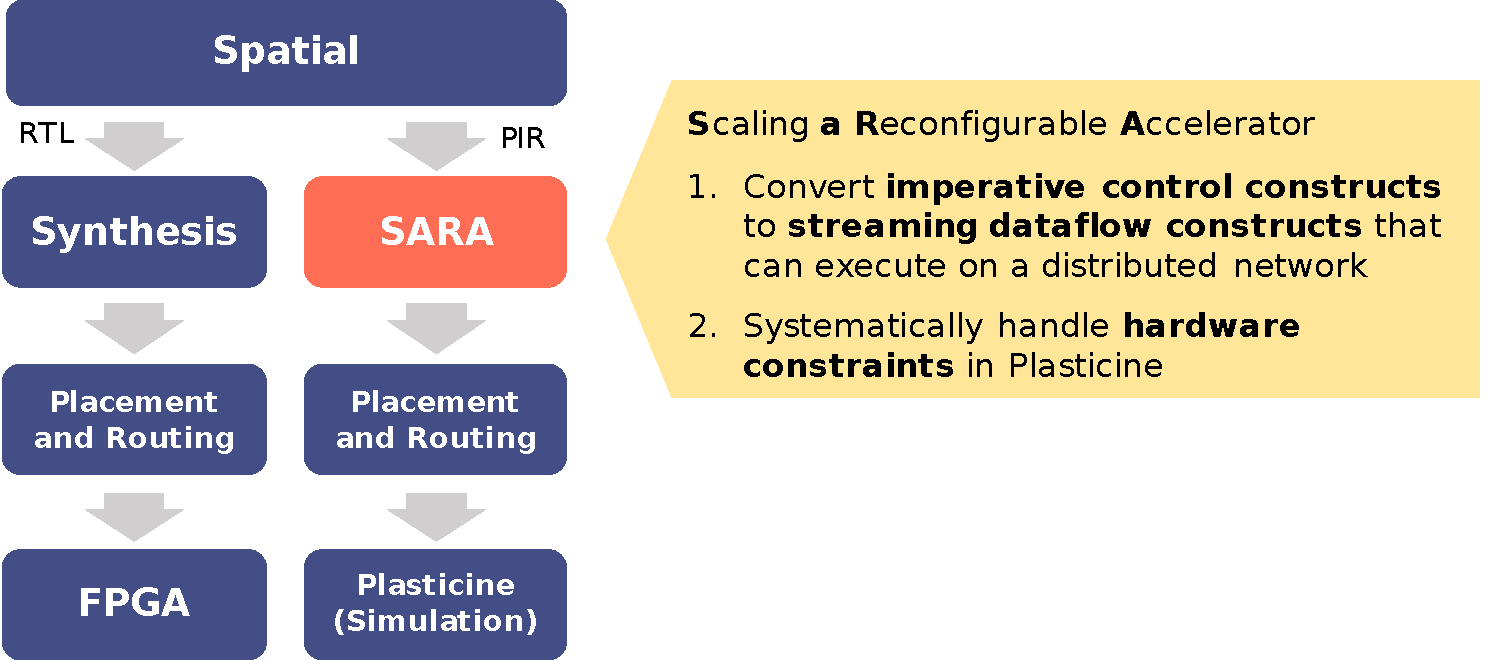
\includegraphics[width=1\textwidth]{figs/spatialstack.pdf}
\caption[Spatial Stack]{Spatial Stack}
\label{fig:spatialstack}
\end{figure*}

Although \name takes Spatial as front-end, the compilation techniques in \name can be equally
applied to other imperative langauges with nested loop constructs, such as C-based high-level
syntehsis language, the backend of Halide IR, and other DSLs at the similar abstraction level. 
Using Spatial as our front-end language has the advantage that the language is designed for
reconfigurable hardware, such that it can express valid execution schedule that can be exploit by
spatial architectures natively in the language.

%% Memory model
The data structure reprsented most exisitng imperative languages IR often marries to the
CPU's virtual memory model. LLVM-based compilers, for example, treats data collections as pointers to a shared
global address space, without distinguising what data are stored on-chip vs. off-chip.
This is CPU provides the memory abstraction that any data within the global address space 
can be equally accessed and the hardware implicitly manage the data movement between on and off-chip 
access by brining
Accelerators on the other hand, has explicitly managed on-chip scratchpads, that is not a cached
version of main memory data implicitly managed by the hardware.
The idea is to have the algorithm, which has better understanding of the data characteristics, to
explicitly control what data gets moved on and off-chip to maximize locality.
Other important static analysis in synthesis compilers, such as banking analysis, requires the
compiler to have the global view all access patterns on a data structure.
Therefore, modeling the data structures as disjoint memory space is much more suitable 
than pointers to a shared memory for reconfigurable architectures.

Without lost of generality, we use python-style pseudo code to represents the front-end programming
abstraction the the rest of our discussion.

Most compilers for CPU uses a control flow graph to represent the control of a imperative program.
The control flow graph implicitly assumes the program is executed in time, which make it unsuitable
for analysis of a reconfigurable architecture that executes the program in space. 
Spatial uses a control hierarchy in the IR to captures the scheduling of the program.
The control hiearchy uses a tree structure to represent the nested control constructs, making it
easier to search the LCA of two controllers.
\Cref{fig:spatialegpar} shows an example of a control flow graph vs. a control hiearchy.
The controller at each level of the hierarchy corresponds to a control primitive, such as a loop, or
a branch statement. 
A basic block is attached to each \emph{inner most} controller including instructions
and memory accesses to user declared data-structures.
If the program has instructions in a outer loop, Spatial automatically inserts a \emph{unit}
controller to wrap the floating instructions.
\name takes the backend of Spatial IR as the input, which is an control hierarchy after loop
unrolling.

\begin{figure*}
\centering
\begin{subfigure}[b]{0.4\textwidth}
\inputminted{python}{code/spatialegpar.py}
\caption{Pseudo Spatial example}
\end{subfigure}
\hfill
\begin{subfigure}[b]{0.58\textwidth}
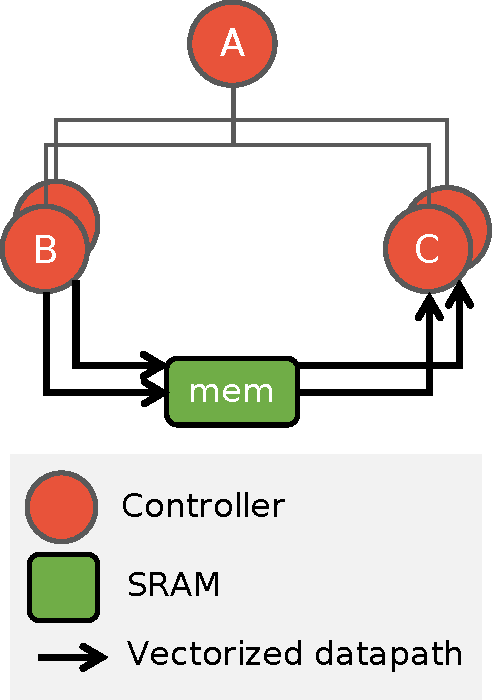
\includegraphics[width=1\textwidth]{figs/spatialir.pdf}
%\missingfigure[figwidth=1\textwidth]{Spatial IR}
\caption{Schematic Spatial IR}
\end{subfigure}
\caption[Spatial Example]{
  Pseudo example of \name's front-end language.
  (a) shows the an example of \name's front-end language. The actual front-end Spatial is a
  Scala-embeded DSL. For simplicity and generality, we use a python style pseudo code to show an
  language with similar abstraction. The `par` keyword indicates outer loop unrolling factor, and
  the `vec` keyword is followed by a inner-loop vectorization factor.
  When an iterator is vectorized, instructions using the vectorized iterator is automatically
  vectorized as well. When unrolling the outer loop \texttt{A}, the enclosed loop body and
  next-level control hierarchy are duplicated, as suggested in (b).
  Each loop in (a) corresponds to a controller in (b). The inner most controllers \texttt{B} and
  \texttt{C} each contain a basic block within instructions within the inner most loops.
}
\label{fig:spatialegpar}
\end{figure*}

